%%% template.tex
%%%
%%% This LaTeX source document can be used as the basis for your technical
%%% paper or abstract. Intentionally stripped of annotation, the parameters
%%% and commands should be adjusted for your particular paper - title, 
%%% author, article DOI, etc.
%%% The accompanying ``template.annotated.tex'' provides copious annotation
%%% for the commands and parameters found in the source document. (The code
%%% is identical in ``template.tex'' and ``template.annotated.tex.'')

\documentclass[conference]{acmsiggraph}

\usepackage{authblk}
\usepackage[]{algorithm2e}

\TOGonlineid{45678}
\TOGvolume{0}
\TOGnumber{0}
\TOGarticleDOI{1111111.2222222}
\TOGprojectURL{}
\TOGvideoURL{}
\TOGdataURL{}
\TOGcodeURL{}



\title{Tracking Objects on a Deformable Surface using Displacement and Orientation Information}

\author[1]{Zachary DeStefano\thanks{zdestefa@uci.edu}}
\author[1]{Kyle Cutler\thanks{kbcutler58@gmail.com}}
\author[1]{Gopi Meenakshisundaram\thanks{gopi.meenakshisundaram@gmail.com}}
\author[1]{Thomas O'Sullivan\thanks{tosulliv@uci.edu}}
\author[1]{Albert Cerussi\thanks{acerussi@apple.com}}
\author[1]{Bruce Tromberg\thanks{bjtrombe@uci.edu}}
\pdfauthor{Zachary DeStefano,Kyle Cutler,Gopi Meenakshisundaram,Bruce Tromberg}
\affil[1]{University of California, Irvine}

\keywords{Tracking, Deformable Surface}

\begin{document}

%% \teaser{
%%   \includegraphics[height=1.5in]{images/sampleteaser}
%%   \caption{Spring Training 2009, Peoria, AZ.}
%% }

\maketitle

\begin{abstract}

For various medical applications, there is a need to track the location of probes as they move across a patient's body. Previous attempts at tracking objects as they move have used magnetic fields or a camera array. These options are impractical for our purposes. Additionally, the surface of a patient's body is deformable. In an attempt to rectify these problems, we developed a probe that produced displacement and orientation data as output. We then came up with an algorithm for taking all that data in real-time and producing a visualization of the path of the probe on the patient's body. 

\end{abstract}



\begin{CRcatlist}
  \CRcat{I.3.5}{Computer Graphics}{Computational Geometry and Object Modeling}{Geometric algorithms, languages, and systems};
\end{CRcatlist}

\keywordlist

%% Use this only if you're preparing a technical paper to be published in the 
%% ACM 'Transactions on Graphics' journal.

\TOGlinkslist

%% Required for all content. 

\copyrightspace

\section{Introduction}

There are various medical device probes that take data at different points on the surface of a patient. It is very important to know the exact location of these points on the surface of a patient. One of the current methods used is attaching a grid to the patient and recording the data at each point in the grid. This process is painstaking and we thus sought a way of automating it. We decided to use motion tracking technology to record the points faster. Using this technology had the added benefit of recording more points than previously. Because the surface of a patient is deformable, simple tracking in 3D would not suffice. We needed a method that would track directly on the surface. Because of that we use an optimal mouse sensor to track the displacement. Mouse sensors do not however tell you how you are oriented so we added a gyroscope, compass, and accelerometer to tell us that. \\
\\
We want to visualize this path in a 3D environment. As a reference then, we do a 3D scan of the patient beforehand and load it into our environment. There will be calibration points marked on the patient before the 3D scan and those will serve as starting points for our tracking. We now have the problem of given this 3D model and a starting point on it as well as the displacment and orientation data, how we do produce an accurate visualization of the path. Because we have a 3D environment, we need to convert the 2D displacement from the mouse sensor and rotation angles from the orientation equipment and output 3D points corresponding to the location of the probe on the virtual surface. \\
\\
Because we have a pre-loaded model to follow, we need to make sure that displacement in the real world is accurately shown as displacement in the virtual world. Additionally, we need to make sure that orientation in the real world matches the one we see in the virtual world. Once that happens, we can start producing 3D paths in the virtual world that resemble the path the probe took in the real world. Because the surface is deformable, we will also have to transform this path so that it directly follows the virtual surface. Once all of this is done we will be able to produce reasonably accurate paths in the virtual world that show the path the probe took in the real world. By coloring the different parts of the path depending on the data taken there, we can also give doctors an accurate picture of which parts of the surface of a patient are important.

\section{Related Work}

\subsection{Mouse Sensor Tracking}

With a typical mouse sensor, $x$ and $y$ displacements are outputted by comparing the images taken by the low-resolution camera at the bottom of the sensor. It thus works quite well a computer mouse since it just needs to lie on a rough surface. With a computer mouse, every movement updates the mouse position for the user and the user only cares about the position in the virtual desktop. There is no consideration for where the mouse is located on the surface and indeed mouse sensors were never designed with that in mind.\\
\\
For our purposes, we want to measure displacement on a 2D surface but we care quite a bit about its exact location on that surface. If the user only moves the mouse horizontally or vertically then we could obtain an accurate location on the real surface easily. However, the probe is bound to be rotated on the surface and when that happens, the axis by which the mouse sensor reads $x$ and $y$ displacement also changes.\\
\\
To overcome the problem of not knowing the orientation of the $x$ and $y$ directions, we could attach a compass to the hardware. That combined system would work well if we were measuring on flat surfaces. However, we are aiming to measure on curved surfaces, thus when the orientation changes, it might be in a direction that a compass could not detect. We thus add an accelerometer and gyroscope to the system in order to get a complete picture of the orientation. 


\subsection{3D Tracking}

Even though we are tracking on a surface we would still need a tracking system that gives us the 3D location of an object. This is due to the fact that our surfaces are arbitrary. 

For our purposes, we needed a tracking system that gave us a 3D location. This is due to the fact that we want to track on a surface but won't know the shape of the surface in advance. Because we do not know its shape in advance, we cannot make assumptions about tracking on it the way we would a 2D plane. Instead we need to acquire 3D coordinates and reconcile them with the surface. \\
\\
Motion capture in the entertainment industry would give us 3D location. Additionally, using a Kinect with a depth map would also give us 3D location. We could have also tried using multiple images to get the sense of depth and acquire a 3D location using that method. All of these ideas however require the object to always be in view of the camera. For the purposes of a clinical setting, that is not practical and we thus needed to explore alternatives. \\
\\
There is currently considerable research on Electromagnetic Tracking for clinical applications \ref{emTrackingReview}. This would give a 3D location for a medical device probe. The systems currently in development do provide millimeter-level precision. These systems have proven to be expensive and difficult to implement. Once our system has been perfected, it would be inexpensive and simple to operate. Additionally, our system guarantees that we are tracking on the surface of a patient which is the main goal of this project. 

\subsection{3D Ultrasound}

There are 3D ultrasound systems **INSERT REFERENCE** which do track on the surface of a patient. It takes ultrasound readings and uses orientation and displacement sensors to help align the readings in order to generate a 3D data set of the inside of the patient. Using this system, orientation and displacement information is combined to generate complete paths. The paper did not consider the exact location on the surface where they placed the probe. They just used the path information to help stitch together the data set. \\
\\
Our technology is meant to use this path information as well as a preloaded mesh in order visualize the path of the probe on the patient. \\
**MENTION 3D ULTRASOUND**\\

The problem of tracking a sensor on the skin's surface was approached in \ref{3dUltrasound}. Much of the initial work on tracking the position of a probe using the orientatation and displacement was inspired by this method. In the paper however they do not deal with the deformability of the surface. This paper attempts to reconcile that problem.\\

\subsection{Human Tracking}

Tracking human motion was approached in \ref{humanMotionTracking}. It figures out a 3D path and integrates orientation and displacement information. It does not reconcile it though with a 3D mesh of the patient. It also does not consider the deformations of the surface of a patient. With our research, we incorporate the deformations. 

\subsection{Deformable Surface Tracking}

Current work on deformable surface tracking is focused on tracking the deformations of the surface itself \cite{deformableobjecttracking,convexopt}. Additionally these works focus on surfaces that do not retain their shape after deformation. For our purposes the surfaces are elastic and thus retain their shape. This paper focuses on surfaces that deform when pressure is applied but then retain their shape afterwards. It is also focused on tracking objects on the surface rather than the surface itself.\\
\\

\subsection{Mesh Unfolding}

Being that we are tracking on a 2D surface embedded into 3D space, we thought about trying to flatten the mesh first and then track on it. We considered using a mesh flattening algorithm that used topological surgery \cite{meshunfolding}. There are other mesh flattening algorithms that exist but in the end we only used mesh flattening for a small neighborhood around where the probe currently was located. Even though the mesh flattening does not have any holes or gaps when using this algorithm, there is no way to assure that our path will not leave the boundary of the flattened mesh. Additionally, we need an algorithm to work on arbitrary meshes and the mesh flattening was only proven to work with a handful of meshes. Due to these difficulties, we decided not to flatten the entire mesh and only do local flattening when we want the path to follow the mesh, which means we care about the triangle where the path is currently as well as its neighboring triangles. 

\section{Tracking Algorithm}

\subsection{Coordinate Systems}

In order to produce an accurate paths for visualization, we have the problem of given 5 values from the probe, $(x_{probe},y_{probe},\theta_{yaw},\theta_{pitch},\theta_{roll})$ and we need to translate that into 3 values for the virtual world, $(x_{virtual},y_{virtual},z_{virtual})$. Here the $x,y,z$ refer to displacements in those directions. We have 4 coordinate systems that we need to consider:\\
\\
1. Mouse sensor coordinate system, subscript $m$\\
2. Probe coordinate system,  subscript $p$\\
3. Real world coordinate system, subscript $k$\\
4. Virtual coordinate system, subscript $w$.\\
\\
The mouse sensor gives us $x,y$ values for each displacement. Thus the positive x-vector corresponds to an $x$ displacement read by the mouse sensor and the positive y-vector corresponds to a $y$ displacement read by the mouse sensor. The negative z-direction corresponds to the direction that the mouse sensor points which in practice will be the direction towards the surface. Thus the positive z-axis will point away from the surface. Due to the nature of the hardware, we can assume that these vectors are orthogonal to each other.\\
\\
The probe gives us orientation data in the form of yaw, pitch, and roll angles. We want to combine this with the $x,y$ data to get the proper displacement vector. We will thus define a probe coordinate system. In this system, the $x,y,z$ vectors are the same as for the mouse sensor system if all the angles are $0$. Also, in this system, the yaw angle means a rotation about the z-axis. The pitch angle is a rotation about the x-axis. The roll angle is a rotation about the y-axis. \\
\\
The real world coordinate system has the units in millimeters and corresponds to displacements from an origin point. The virtual world will be virtual displacements from an origin point on the scanned model. For the sake of the simplicity, the $x,y,z$ directions in the real world system will be the same as in the virtual world system. The point of keeping track of the real world coordinates will just be scaling the displacements. 

\subsection{Rigid Coordinate System Transformations}

There are a few assumptions we can make that simplify the process of converting between coordinate systems. All of the basis vectors are orthogonal in each of the coordinate systems. Therefore any conversions between them is an orthogonal matrix. Every orthogonal matrix is the product of one rotation and one reflection, which simplifies the process of finding out which orthogonal matrix will do the conversion we need. \\
\\
We also have rigid motion so the probe coordinate system and the virtual coordinate system stay constant. Additionally, any changes in the probe's position only come from the $x,y$ data. The angle data only gives us the orientation when there is a change in position registered. This means that we can equivalently formulate the problem as taking the $x,y,z$ vectors from the mouse sensor space and finding their equivalent orthogonal vectors in the virtual space given particular $\theta$ values for the angles. If there is a reflection then, it would only be one about the $y-z$ plane to flip the x-axis or about the $x-z$ plane to flip the y-axis. \\
\\
Now that we have scaling, we only have to worry about direction. The map from the mouse sensor coordinate system to probe coordinate system is not a static map. It is a transformation that depends on the orientation angle reading from the probe. In this system, the yaw angle means a rotation about the z-axis. The pitch angle is a rotation about the x-axis. The roll angle is a rotation about the y-axis. \\
\\
We use an Euler Angle to Quaternion conversion to get the rotation we should apply to the mouse sensor coordinate system in order to obtain coordinates in the probe coordinate system. The API that we used had a method \cite{jmonkeyrotation} and the logic used in the method is a common one to go from Euler Angles to Quaternions \cite{quaternionTextboook}.

**MENTION THAT CALIBRATION OBTAINS THE ORTHOGONAL MATRICES THAT ENSURES GOOD TRANSFORMATIONS BETWEEN COORDINATE SYSTEMS**

\subsection{Building Paths on the Mesh}

**BRIEFLY MENTION THE PATH RECORDING ALGORITHM**\\
\\
Due to the nature of the recording, we need a way to compress the vertex list to be meaningful so all the vertices are distinct and no segment is too little. This is the algorithm I used: \\
**INSERT COMPRESSION ALGORITHM**\\
\\
**MENTION NEED FOR MESH FOLLOWING ALGORITHM**\\
\\
**MENTION HOW 3D SCAN IS INCORPORATED INTO VIRTUAL WORLD AND THE PATH RECORDED IS RECONCILED WITH THE SURFACE**

\subsection{Tracking System Components}

\subsecton{Tracking Protocol}

\section{Mesh Traversal Algorithms}

\subsection{Following a Deformable mesh}

For the purposes of our application, we need to have paths on the mesh itself so that we know the location on the mesh of particular data points. Due to the deformability, the paths ends up being close to the mesh, but not on the mesh itself, no matter how accurate the calibration was. Additionally, in order to do the calibration, we need the path to follow the mesh itself so that the end points line up. We thus came up with an algorithm for projecting a path onto the triangles of the mesh. \\
\\
A path is just a series of connected segments and the mesh is just a series of triangles. Thus the input of our algorithm is a segment with a start and end point as well as the triangle where it originates and the triangles neighbors. We need to make sure the projection preserves the length of the segment. We also want to preserve the orientation along the surface thus we are restricted to rotating the segment along the plane that it makes with the triangle's normal. \\
\\
If we let $v$ be the segment vector, $N$ be the normal, and $E$ be the resultant vector that is the projection of $v$ onto the plane described by $N$, then the following equation will get us $E$
\[
E = v - proj_N(v)
\]
This can be furthur simplified to say
\[
E = v - N(v.N)
\]
We then find the intersection of the vector $E$ with the current triangle. If the segment is entirely in the triangle, then we move onto the next segment starting from the endpoint of $E$. If the segment leaves the triangle, then we find which edge the segment intersects and repeat the projection procedure for the end part of the segment that is not in the triangle. This procedure of course relied on finding the intersection of the triangle with the segment which proved to be non-trivial.\\
\\
When finding the triangle and segment intersection, we had a triangle in a 3D space as well as a segment that was supposed to be coplanar to the triangle but could be slightly off due to floating-point errors with the coordinates. To find the intersection point, I converted the segment and triangle coordinates to the coordinate system where one of the vertices of the triangle is the origin and the basis vectors are the two vectors made by the segments coming off that vertex as well as the cross product of those vectors. In this coordinate system, the third coordinate should be zero. In practice, it was near zero due to floating point errors. Once in the new coordinate system, we just had to find the 2D intersection of the triangle and the segment. \\
\\
The above procedure describes what we did with a single segment. With paths, we just iterated this procedure for each segment of the path. We assumed that the important aspect of each segment is its vector and not its origin point, since that is what we get from the probe. This meant that the end point of a projected segment was treated as the start point for the rest of the path when doing the loop to project the entire path onto the mesh.

\subsection{Calibration of Rotation and Scale}

After taking a 3D scan and importing the mesh into our environment, we have our object in a virtual world with a virtual coordinate system. Our probe operates in the real world. We thus need to know how to translate between the two in order to get an accurate visualization. We first needed to translate displacement readings from the probe to displacement in the virtual world. Afterwards, we needed to get rotation and reflection calibrated so that the displacement vectors went in accurate directions in the virtual world. \\
\\
The Scale Calibration was relatively straightforward. The probe gave numerical displacement readings that ranged from -127 to 127. We then made the probe travel 100 mm in every direction and summed up the displacement values. This gave us a probe unit to millimeters conversion factor. We then measured the distance between the calibration points in the virtual world and in the real world in millimeters and this gave us a virtual unit to millimeters conversion ratio. We then combined the two ratios and obtained a probe unit to virtual unit conversion ratio. \\
\\
The Rotation Calibration was difficult. This involved recording a path that went between calibration points and finding the correct rotation to apply in the virtual world so that the start and end point of the path are the points on the mesh. Making the start point match is easy as you just translate the path. With making the end points match, the path has to follow the mesh in order to conclude that the end points truly match. We needed to find a rotation to apply to the path that would make end points match as close as possible while the path is projected onto the mesh. In order to do this, I first rotated the path onto the mesh meaning the first segment of the path was on the same plane as its triangle. I then rotated the path along the plane made by the first triangle until the end points matched up closely. I then took the rotated path and projected it onto the mesh. I then found the rotation required to match the projected path endpoint with the target endpoint. I used that angle and rotated the original rotated path along the surface that much. I then projected that path and repeated the process until I got convergence. The aggregate rotation that resulted was used as the rotation calibration and applied to the rotation found by the probe to get the rotation in the virtual world. Here is the pseudo-code for the rotation calibration:

\begin{verbatim}
N: normal to the first triangle
P: original path
P': current path rotated
P'': the path P' projected onto the mesh

Rotations will be in axis-angle form as (T,E) 
where T is the angle and E is the axis

1. Let p be the projection of the first segment of P onto the first triangle
2. Rotate P so that its first segment matches p and call the rotated path P'
3. Find the rotation (Theta,E) that will make the end point of P' 
   match the target end point
4. Apply the rotation (Theta,N) to P' to rotate it along the 
   same plane as the first triangle
5. Find the path P'' which is P' projected onto the mesh
6. Find the rotation (Theta,E) that will make the end point 
   of P'' match the target end point
7. Apply the rotation (Theta,N) to P'
8. Repeat steps 5-7 until P' converges

Output the quaternion Q such that P' = Q*P

\end{verbatim}

\section{Calibration Steps}

\subsection{Scaling calibration}

In order to do scale calibration, I just consider $x,y$ displacement without any angles being involved. In order to simplify the calibration factor, I find two linear transformation $S_1,S_2$ such that 
\[
S_1(x,y,0)_m = (x,y,0)_k
\]
\[
S_2(x,y,z)_k = (x,y,z)_w
\]
For $S_1$ we only care about $x,y$ scale, so it is a diagonal matrix. We measure a certain distance in the real world and find out the total displacement in probe coordinates. We repeat this for both $x,y$ and this allows us to get $s_{1x},s_{1y}$, the scale factors for $x,y$ respectively. \\
\\
For $S_2$, we are assuming that the real world and virtual world are scaled uniformly. Therefore, we measure the euclidean distance between points in the virtual world and points in the real world and assume that the factor we get can be uniformly applied to the 3 coordinates. Once we get that factor $s_2$, we make $S_2$ as the diagonal matrix with only $s$ on the diagonal. \\
\\
We then find $S=S_2S_1$ although order does not matter since we have diagonal matrices. This gets us $s_x=s_{1x} \cdot s_2$ and $s_y=s_{1y} \cdot s_2$ which are the scale factors to go from probe coordinates the virtual coordinates with $x$ and $y$. We will now let
\[
(x',y',0)_m = S(x,y,0)_m = (x \cdot s_x, y \cdot s_y, 0)_m
\]

\subsection{Rotation and Reflection Calibration}

Now that the scale is calibrated and we have a direction for the displacement, the rest of the process of changing coordinates involves converting one set of orthogonal unit vectors to another set of orthogonal unit vectors, which is just a rotation and reflection. We are given the following at a single point, A, in order to convert between coordinate systems:\\
1. The normal to the plane in both probe and virtual coordinates\\
2. A path from A to a point B on the surface in probe and virtual coordinates\\
3. A path from A to a point C on the surface in probe and virtual coordinates. The AC line should be perpendicular to the AB line. \\
\\
To reconcile 1, we just have two vectors, so we can come up with a rotation matrix $R_1$ to go from one vector to another. This means that one of the unit vectors has been reconciled. \\
\\
To reconcile 2, we just have to rotate the path along the normal until the desired path and the recorded path have the same end point on the surface **INSERT DETAIL**. This will give us a rotation $R_2$. \\
\\
We now have 2 out of the 3 vectors and in order for the unit vectors to stay all orthogonal, there are only two choices with regards to the third vector. We thus have to reconcile 3 in order to see if the positive or negative direction is better. We follow the same procedure as in 2 in order to get the new path but then we see if the reflection will work well. This gives us a reflection matrix $K$ which is the reflection of the $x$ or $y$ axis at the original point.

\section{Implementation Details}

Our process started with taking a 3D scan of the surface to get the mesh. After creating and refining the 3D mesh, we loaded it into a video game style environment that allowed us to produce live updates. Every few milliseconds we obtained displacement and orientation readings from the probe and we used those to update the visualization of the location of the probe in the virtual environment. In order for this to work properly, we needed to know how to convert between the displacement readings from the probe and the displacement in the virtual world. We also needed to know how to convert between the rotation read by the probe and the rotation that corresponds to in the virtual world. Finally, due to the deformability of the surface, we needed an algorithm to approximate the probe's location on the surface in the virtual world.\\
\\
**SHOW PICTURE OF PROBE IN REAL WORLD**\\
**SHOW PICTURE OF PROBE IN VIRTUAL WORLD**

We use a Kinect to get the data and then used software that worked on top of the Point Cloud Library \cite{pointcloudlibrary} to take the data and get a mesh and texture from it. We then edited the mesh using Meshlab \cite{meshlab}. We took out some of the noisy areas and using the Quadric Edge Collapse Decimation filter, which is an implementation of QSlim \cite{qslim}, to refine and simplify the mesh. After that, we load the mesh into our tracking environment. Our tracking environment is an application that takes in the mesh as well as probe data readings and gives live updates as to the probe's position and data. It operates similarly to a video game and was developed using JMonkeyEngine **INSERT DETAIL**, a video game library written in Java that is similar to Ogre **INSERT REFERENCE**. \\
\\
Once the scale is calibrated we know that we have accurate displacements. We know need to ensure that the displacement goes in the right direction. The orientation data from the probe gives us a set of orthogonal vectors. We then need to transform this set into the virtual world.\\
\\
Once the scale is calibrated, we start recording paths on the mesh itself. We then have a problem. Because the rotation has not been calibrated, it is likely that the paths will have a shape similar to the part of the mesh they were on but they will not actually be on the mesh **INSERT PICTURE OF THIS**. We thus need to figure out what rotation to apply to the probe reading's rotation in order to get the rotation in the virtual world. After that though, there is still a problem. Because the surface is deformable, the path would still not perfectly follow the mesh. We thus need an algorithm that will approximate the probe's position on the mesh given the deformability. \\
\\
This paper presents two algorithms. The first one takes a path that almost follows the mesh and projects it onto the mesh in such a way that preserves its orientation along the mesh as well as its arc length. The second one takes a recorded 3D path between two known points on the mesh and figures out how to rotate it and project it onto the mesh so that its start and end points match the ones on the mesh. The rotation found by the second algorithm gives us the rotation calibration we need. Once the rotation is calibration is found, we can then live track the probe and use the first algorithm to keep it along the mesh. 


\section{Tracking the Probe on a Deformable Surface}

\subsection{Mesh Following Algorithm}

After calibration, due to deformability and possible measurement errors, our rendered path in the virtual world will have segments that are above or below the virtual surface as shown in Figure \ref{pathsAboveAndBelow}. Because the path was recorded on the real surface, we want a visualization on the virtual surface of the probe's location on the real surface. We will thus do a transformation of the virtual path to better match where the real path traversed. Because we already calibrated the scale of the movements, the transformation will preserve arc length. Because the rotation was already calibrated, the orientation along the surface will be preserved.

\begin{figure}[ht]
\centering
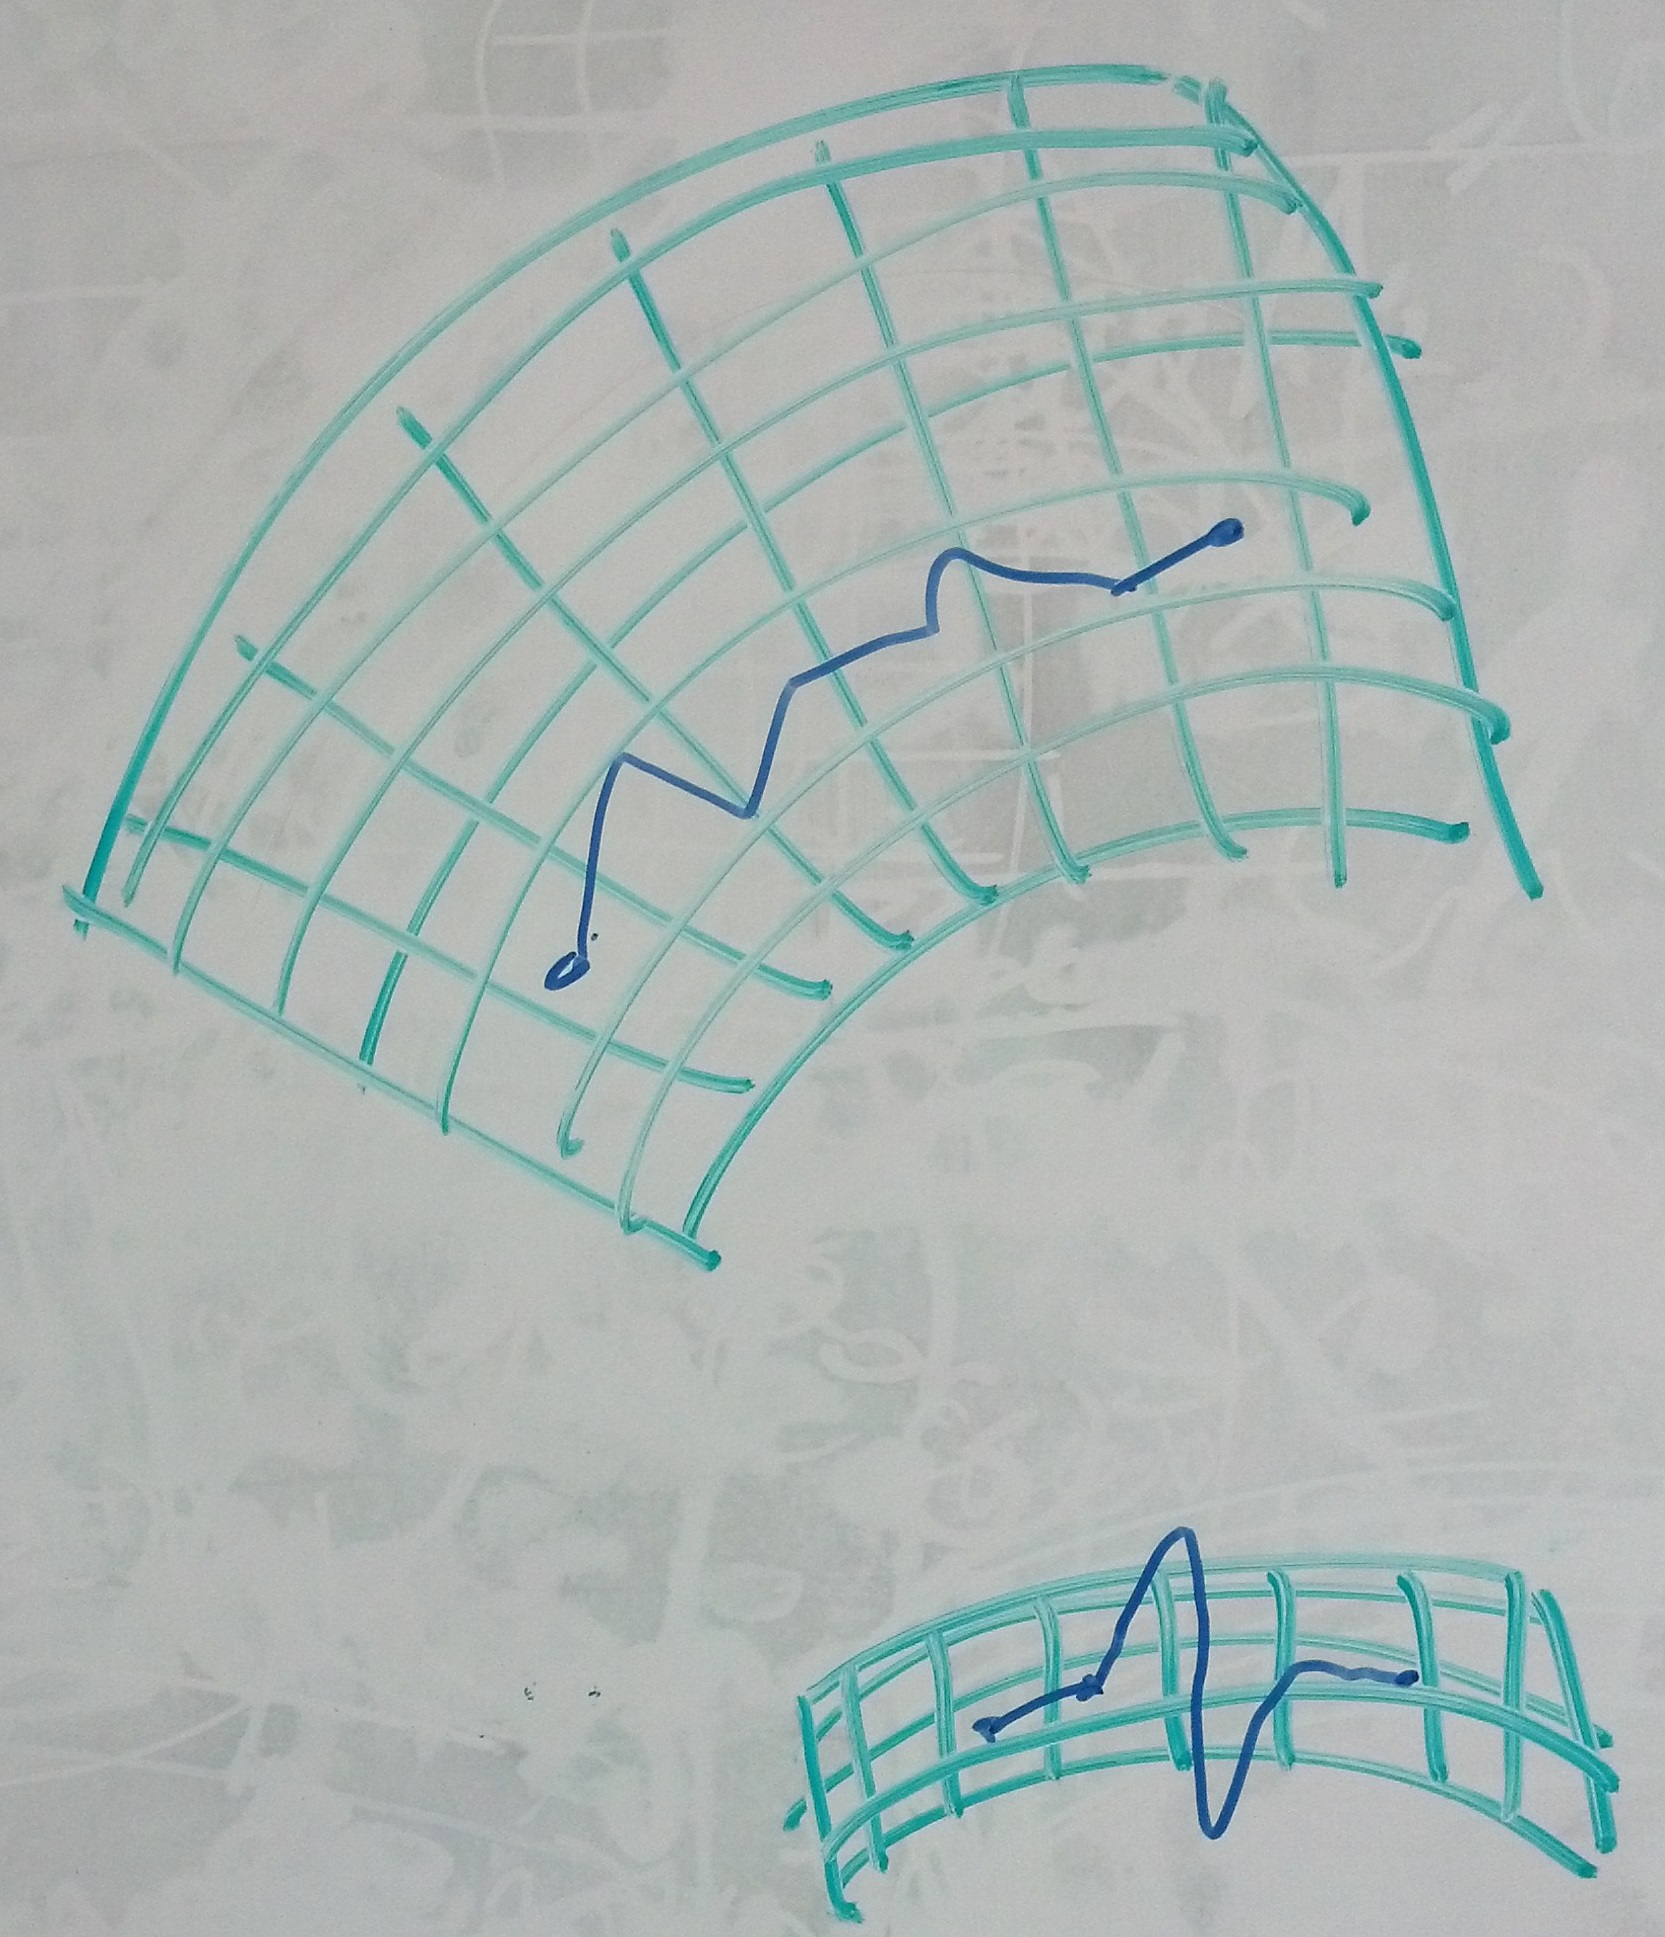
\includegraphics[width=\columnwidth]{pathaboveandbelow.jpg}
\caption{Path above and below surface}
\label{pathsAboveAndBelow}
\end{figure}

We have a known and rigid starting point $p_0$ on the triangular manifold mesh $M$ for our path (TODO: The fact that it is a triangular manifold mesh will be established in previous sections). The rest of the path is a set of $n$ segments $s_0,...,s_{n-1}$ where the starting point of $s_0$ is $p_0$ and the rest of the segments start at the point where the previous segment ended. We need a new set of segments that all lie on triangles of the mesh. Our goal is thus a new path consisting of $m$ points, $p_0, p_1,...,p_{m-1}$, such that each $p_i$ is on $M$ and for each $i>0$, $p_{i}$ and $p_{i-1}$ lie on the same triangle. \\
\\
Once the first segment is transformed to follow the mesh, we will have a new point $p_j$ on the mesh where the first segment ends and the second segment begins. Because each segment starts where the previous one ended, we will transform the second segment using $p_j$ as its starting point. By this same logic, we can repeat this procedure for the rest of the segments. We thus need to focus now on how to transform a single segment with a starting point to points on the mesh making sure to preserve length and orientation along the surface. \\
\\
When we transform a segment, it needs to follow a straight-line path in its direction for its length, thus it should follow the geodesic path along the surface. We will therefore flatten the mesh around the local area that the segment traverses. Let $\epsilon$ be the length of our segment and $p$ be its starting point. The $\epsilon$-neighborhood around $p$ will be homeomorphic to $R^2$, as illustrated in Figure \ref{manifolddiagram}, thus when we flatten the neighborhood, there will be no gaps or overlaps. We will denote $T$ as the triangle where the starting point lies. We will develop a secondary mesh $M_0$ that consists of $T$ and the triangles that intersect the $\epsilon$-neighborhood of $T$. The triangles in $M_0$ will be rotated so that they lie on the same plane as $T$. \\
\\
We now have a vector and a flat plane it needs to follow. We will let $v$ be the vector for our input segment, $N$ be the normal of that plane. In order to preserve orientation along the plane, we need to find a vector $E$ that is both on the plane formed by $N$ and $v$ and has an acute angle with $v$. As can be observed in figure \ref{vectordiagram}, the following equation will then hold
\[
E + proj_N(v) = v
\]

\begin{figure}[ht]
\centering
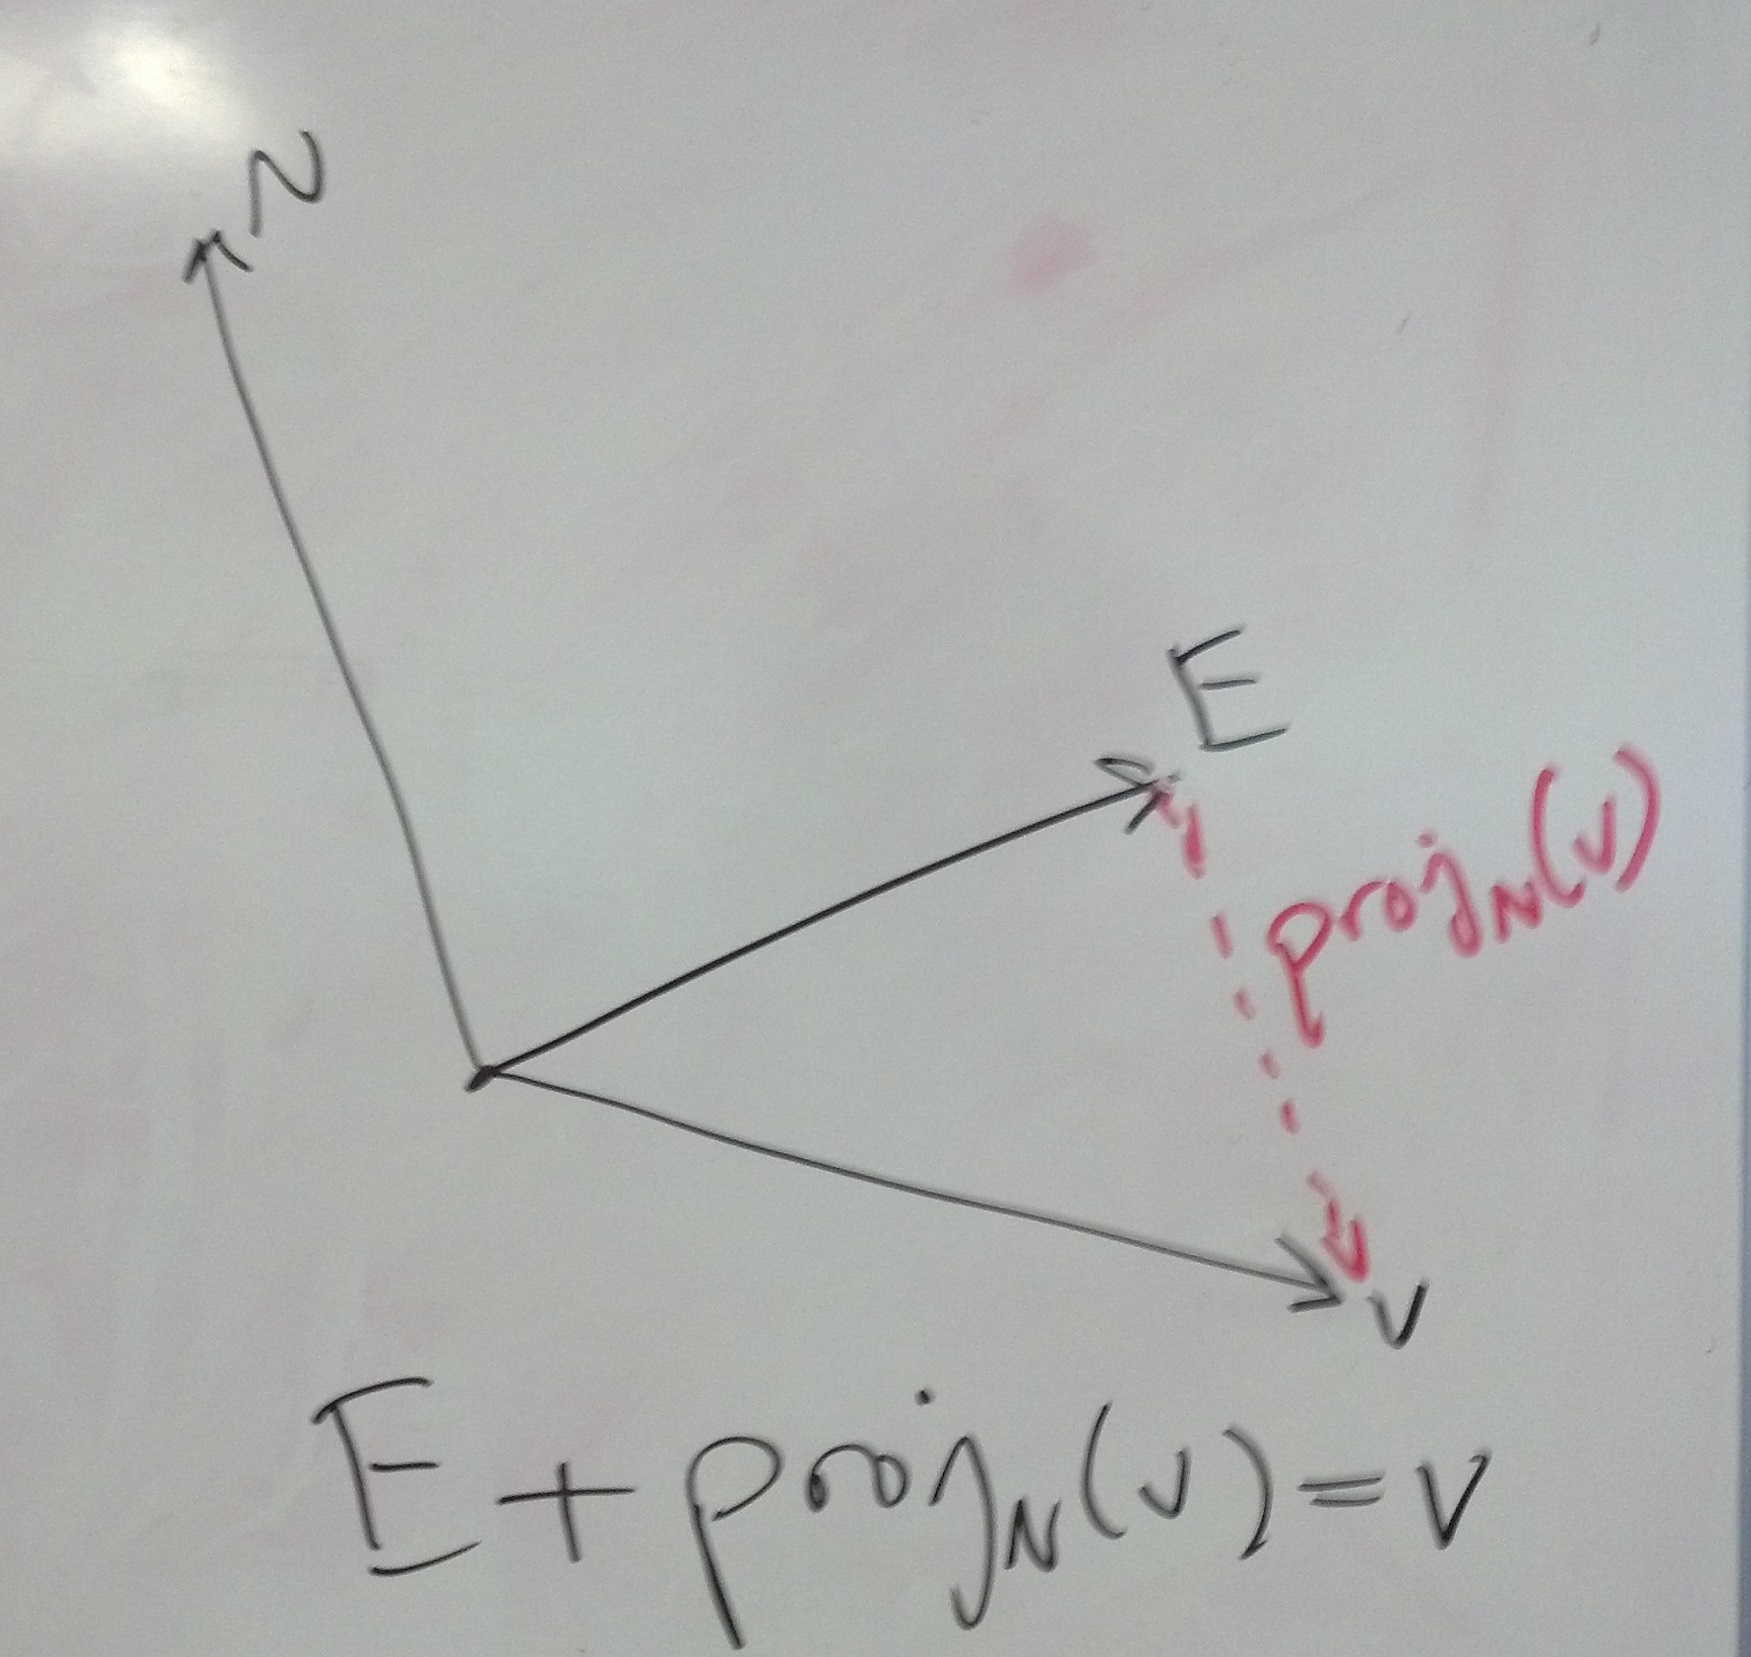
\includegraphics[width=\columnwidth]{vectordiagram.jpg}
\caption{The segment vector, normal, and projected vector}
\label{vectordiagram}
\end{figure}

Thus we can easily calculate $E$ using the formula
\[
E = v - N(v.N)
\]
We will now let $p' = p+E$ which will be the ending point on $M_0$ of our segment. We then take the $p-p'$ line segment and calculate its intersections with edges of the triangles in $M_0$, denoting that set as $Q'$. The points $p$ and $p'$ will also be calculated in their own triangle's coordinate system. The points in $Q'$ that lie on edges between triangles will be calculated in the coordinate systems of both triangles. By finding the point coordinates in the triangle's coordinate system, we can easily transform the $p-Q'-p'$ set of points into the set $\{p_0,...,p_j\}$ where each of those points lie on the mesh $M$. As a summary, the pseudo-code of the algorithm is presented in algorithm \ref{pseudocode}. \\
\\
\begin{algorithm}[t]
Input: Starting point $p_0$, Segments $s_0,...,s_m$, Mesh $M$\;
Set $p \leftarrow p_0$ \;
Initialize list $P$ of points and add $p_0$ to it \;
Set $T$ to be the triangle of $p_0$ \;
\For{each segment $s_i$ in order}{
	Set $N$ to be normal for $T$\;
	Set $\epsilon \leftarrow length(s_i)$ \;
	Set $M_0$ equal to triangles which intersect the $\epsilon$-neighborhood around $p$ \;
	Flatten $M_0$ so its global normal is $N$ \;
	Set $v$ to be the vector for $s_i$ \;
	Set $E \leftarrow v - N(v.N)$ \;
	Set $p' \leftarrow p+E$ \;
	Set $Q'$ to be intersections of $p-p'$ segment with triangle edges in $M_0$ \;
	Transform $p$,$Q'$,$p'$ back to points on M and add them to $P$ \;
	Set $p$ to transformed $p'$. \;
	Set $T$ to triangle at $p'$ \;
}
\caption{Pseudo-code for our algorithm}
\label{pseudocode}
\end{algorithm}

\begin{figure}[ht]
\centering
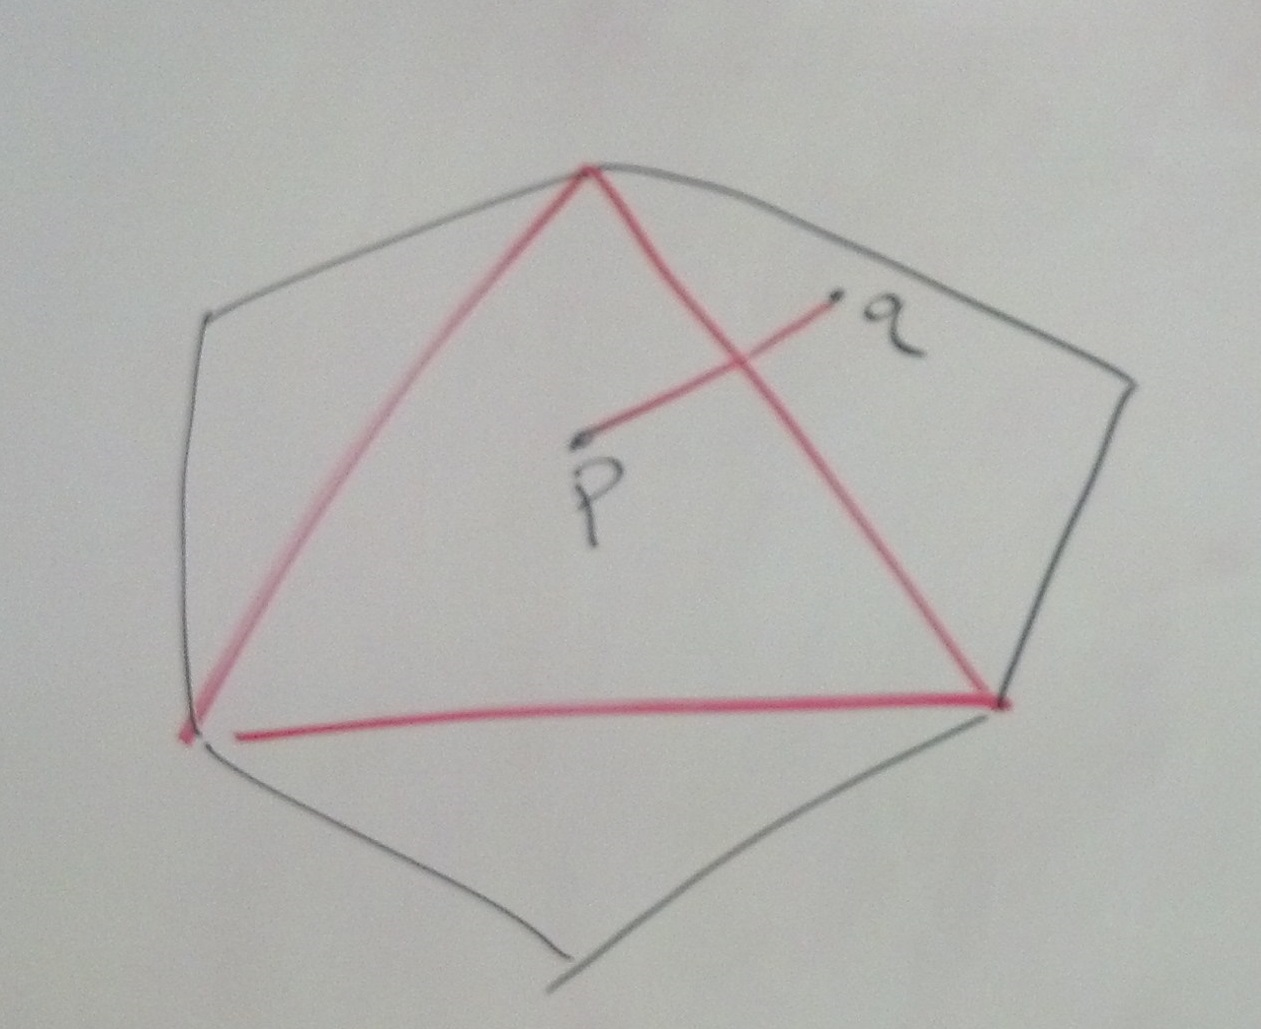
\includegraphics[width=\columnwidth]{flatteningdiagram_oneTriangleAndNeighbors.jpg}
\caption{The triangle at $p$ and its neighbors}
\label{flatteningDiagram_oneTriangle}
\end{figure}
\begin{figure}[ht]
\centering
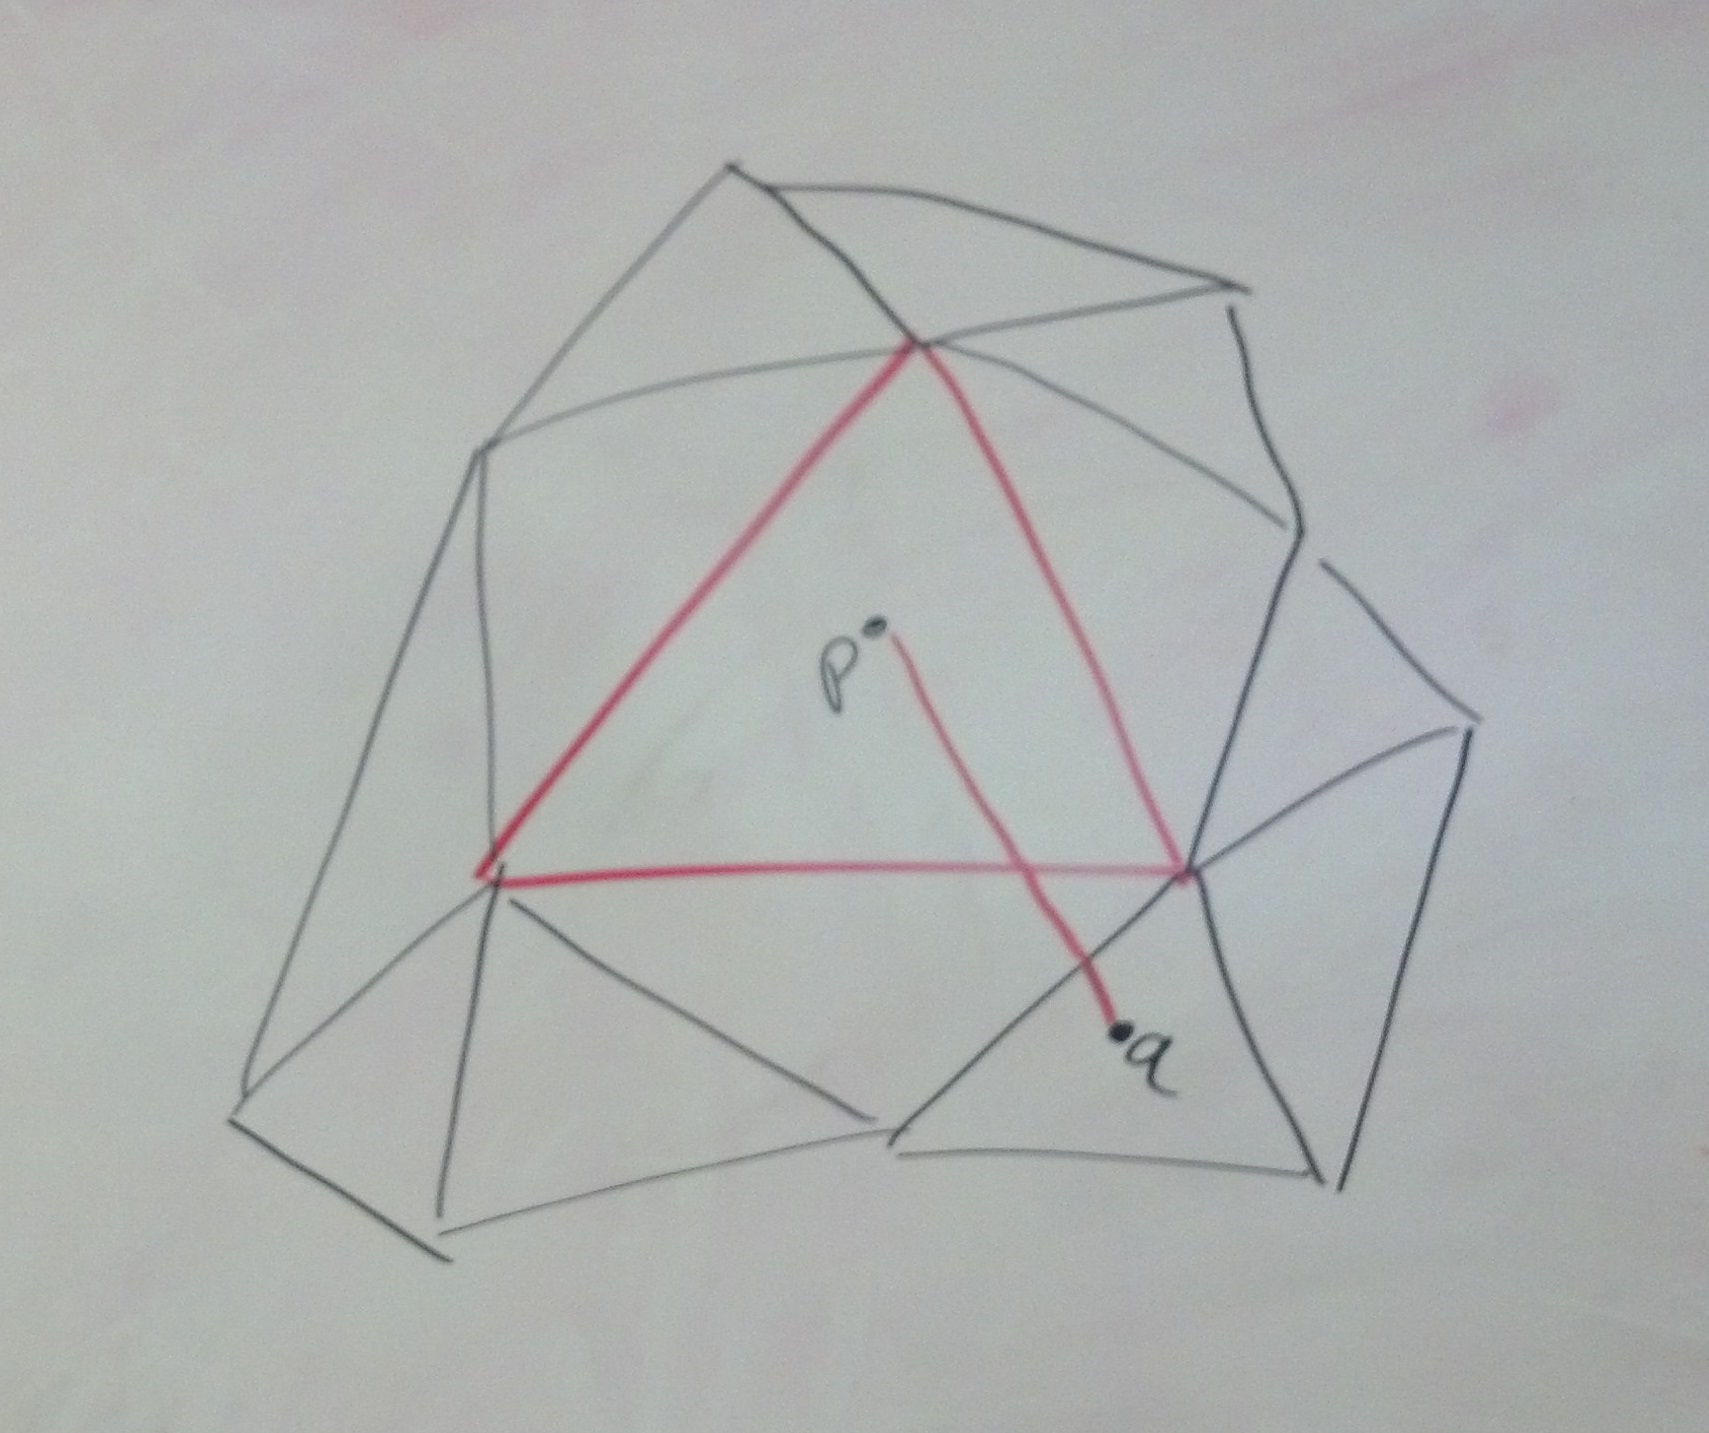
\includegraphics[width=\columnwidth]{flatteningdiagram_neighborhood.jpg}
\caption{The triangles in the neighborhood around $p$}
\label{flatteningDiagram_neighborhood}
\end{figure}

\begin{figure}[ht]
\centering
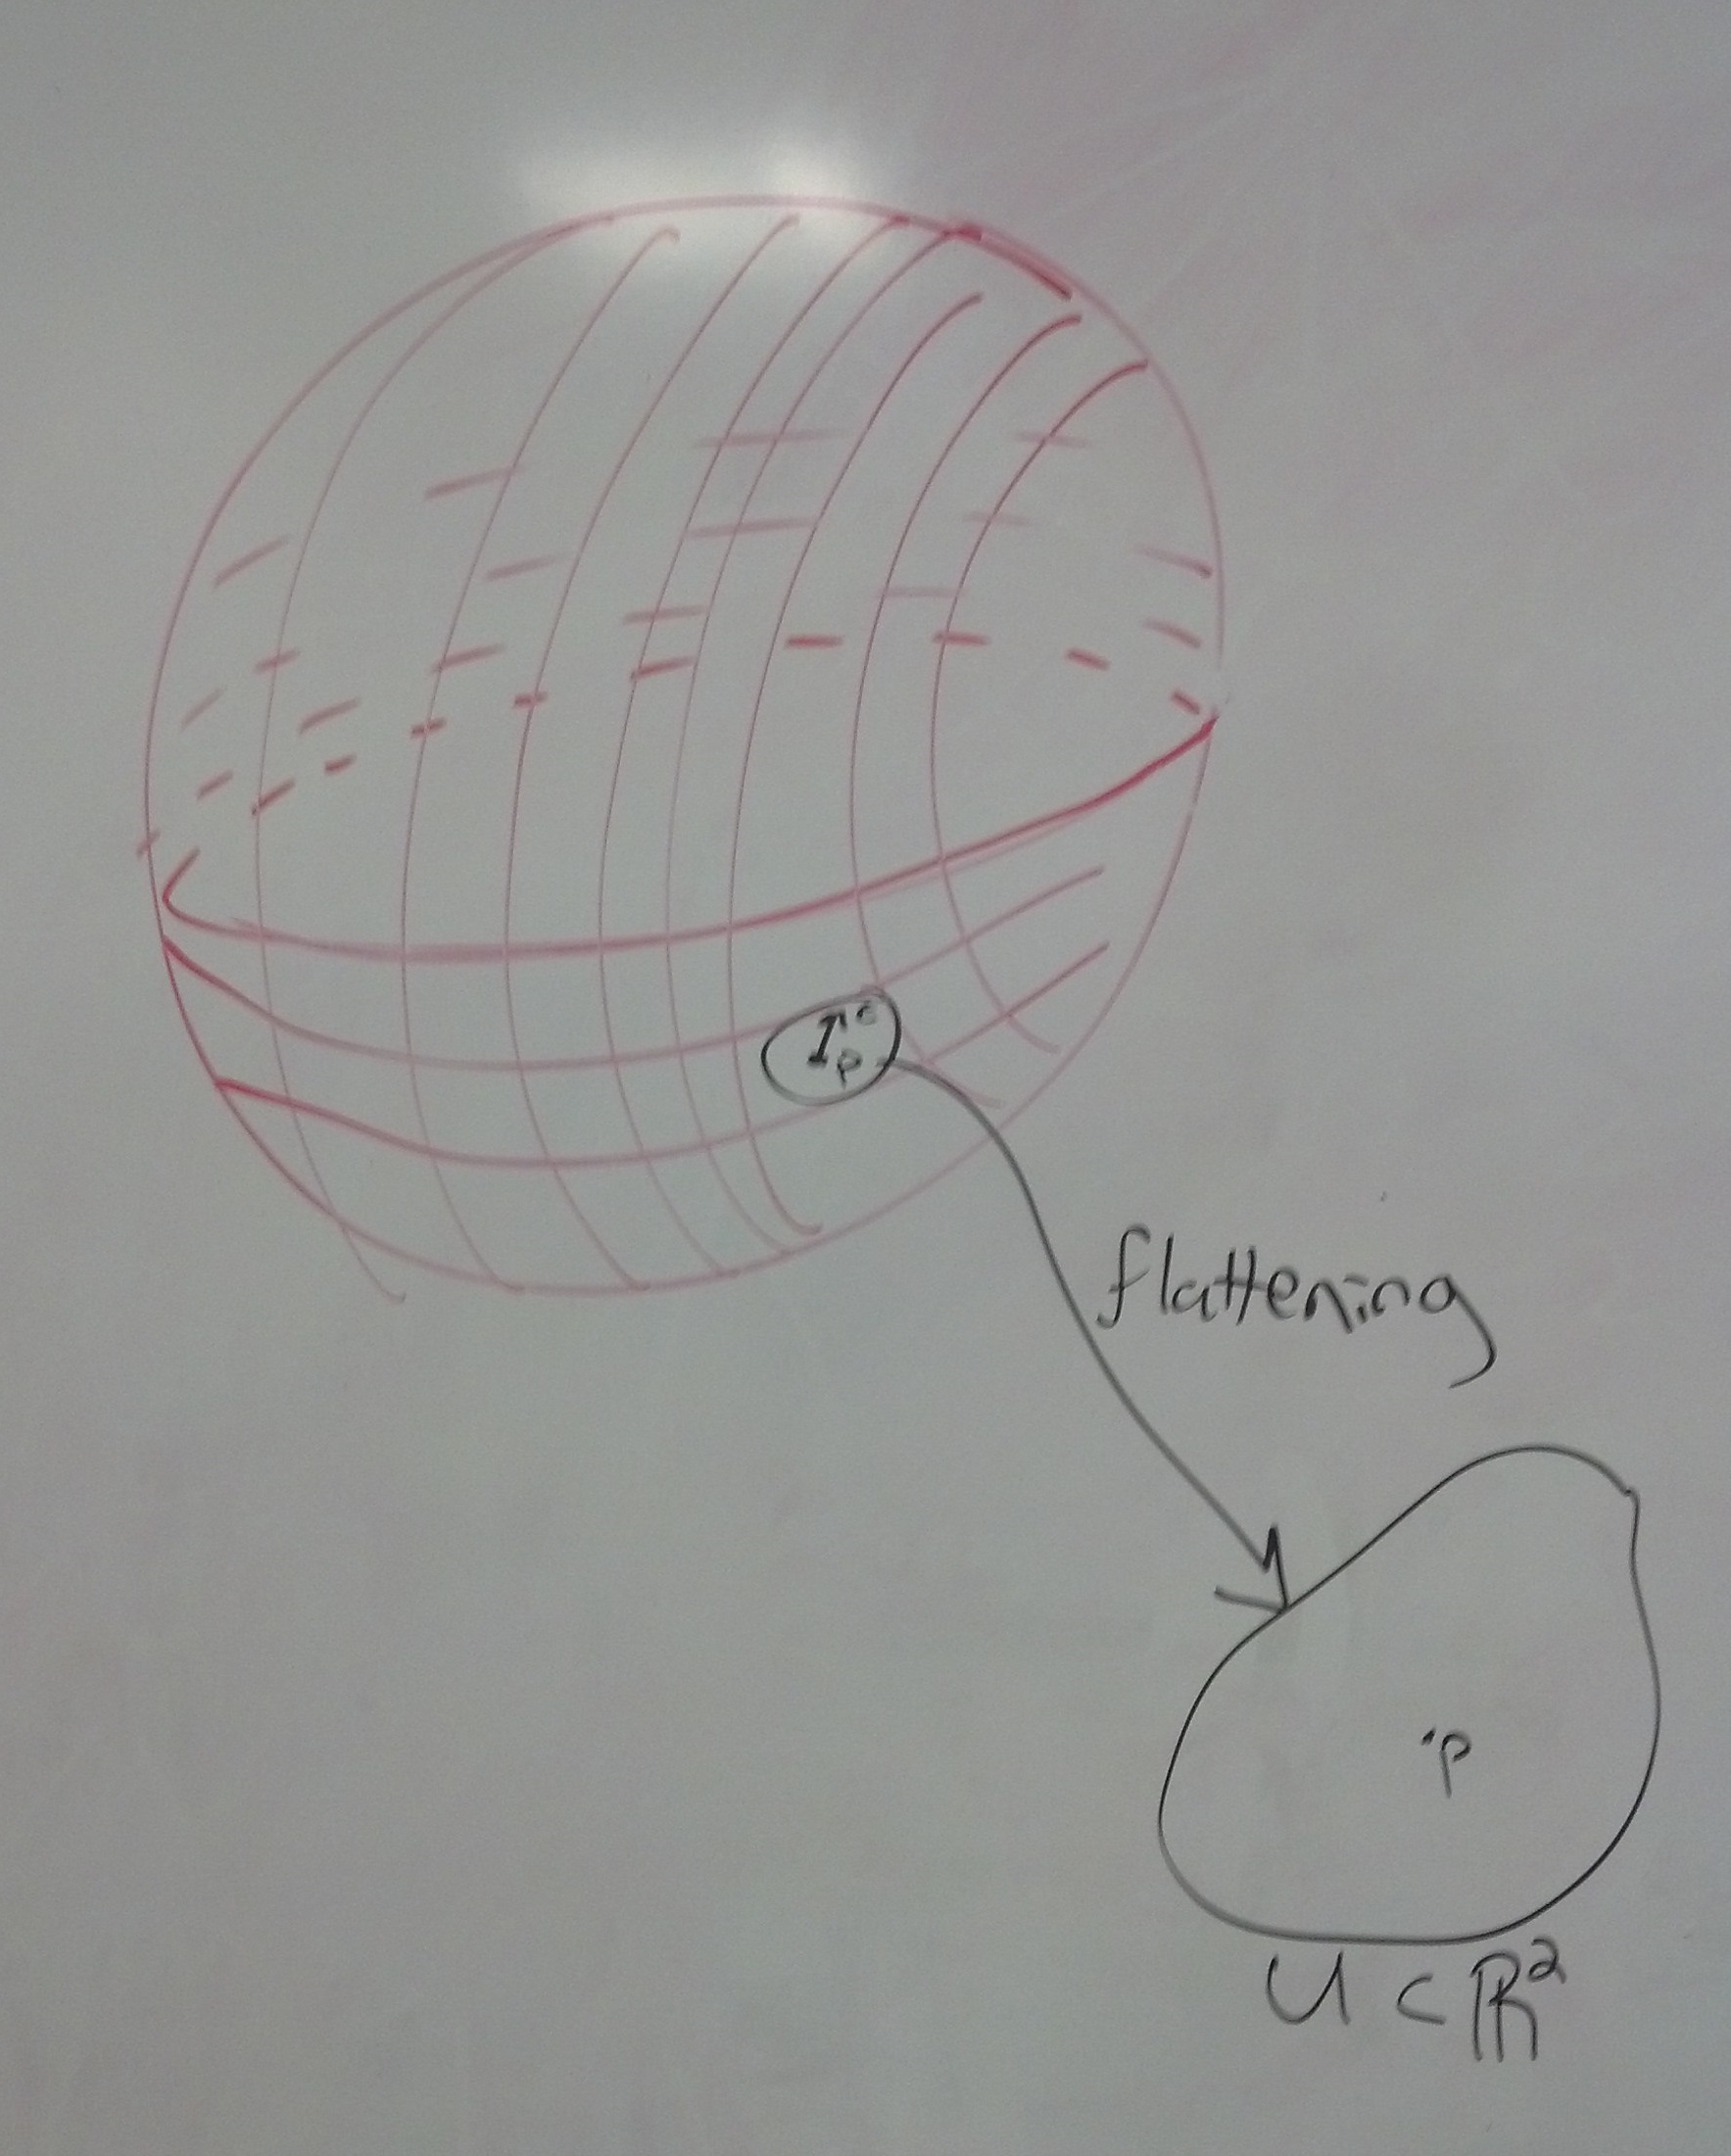
\includegraphics[width=\columnwidth]{manifolddiagram.jpg}
\caption{The manifold with its $\epsilon$ neighborhood at a point $p$}
\label{manifolddiagram}
\end{figure}


\section{Average Error Argument}

Let $x,y$ be the error amounts. Let $\epsilon_x$ and $\epsilon_y$ be the max error for both, thus we care about the range $x \in (-\epsilon_x,\epsilon_x)$ and $y \in (-\epsilon_y,\epsilon_y)$. Let $A$ be the measured value for the $x$ variable and $B$ be the measured value for the y variable.\\
\\
The error is as follows
\[
E(x,y) = |\frac{A + x}{B + y} - \frac{A}{B} |
\]
To get the average, you need to integrate this over the range of $x$ and $y$\\
We need to split this into two regions depending on whether the abs value fraction is positive or negative. \\
In the region $y < \frac{B}{A} x$, the term inside the absolute value is positive\\
In the region $y > \frac{B}{A} x$, the term inside the absolute value is negative\\

\section{Conclusion and Future Work}

This proved to be a good first step and proof of concept for tracking on a deformable surface using simple hardware. Once the process is refined, there are numerous applications to this hardware and software combo. 



%\begin{figure}[ht]
%\centering
%\includegraphics[width=3in]{examplePic_startingProblem.png}
%\caption{Data Units with varying access requirements}
%\end{figure}


\bibliographystyle{acmsiggraph}
\bibliography{trackingRefs}

\end{document}
